\mode*
\section{Mehrdimensionale Funktionen}

\begin{frame}{Arten mehrdimensionaler Funktionen}
\begin{enumerate}
    \item Funktionen einer Variablen, die in $\R^n$ abbilden (Wege):
    \begin{gather*}
        \vf\colon \R\to \R^n,\qquad t\mapsto \vf(t)
    \end{gather*}
    \item Funktionen mehrerer Variablen, die nach $\R$ abbilden:
    \begin{gather*}
        f\colon \R^m\to \R,\qquad \vx \mapsto f(\vx)
    \end{gather*}
    \item Funktionen mehrerer Variablen, die in $\R^n$ abbilden:
    \begin{gather*}
        \vf\colon \R^m \to \R^n,\qquad \vx \mapsto \vf(\vx)
    \end{gather*}
\end{enumerate}
Notation: wir schreiben Vektorgrößen als $\vx,\vy,\vf$ zur Unterscheidung von Zahlen $t,x,f$.
\end{frame}

\subsection{Darstellung}

\begin{frame}{Höhenlinien}
  \begin{center}
    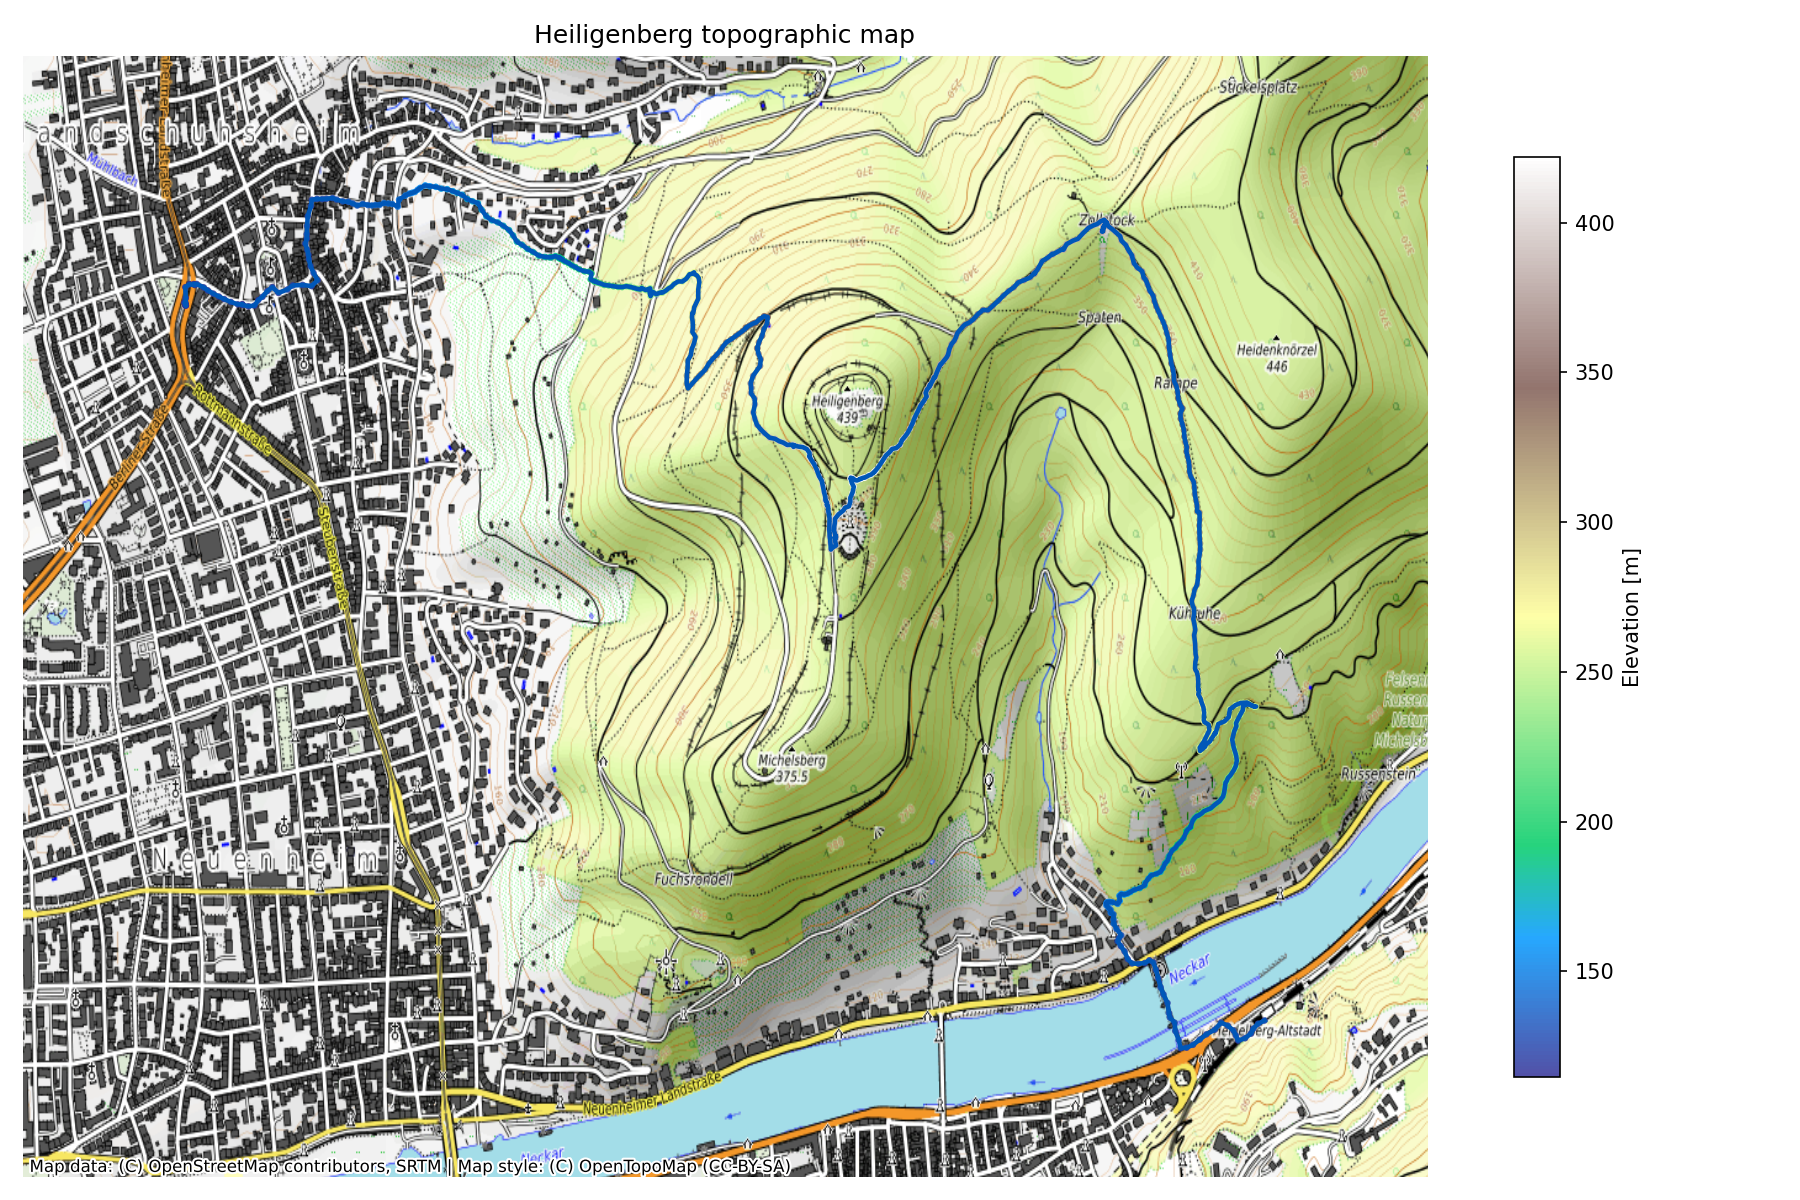
\includegraphics[width=.9\textwidth]{pic/topography_map}
  \end{center}
\end{frame}

\begin{frame}{Oberflächendiagramm (surface plot)}
  \begin{center}
    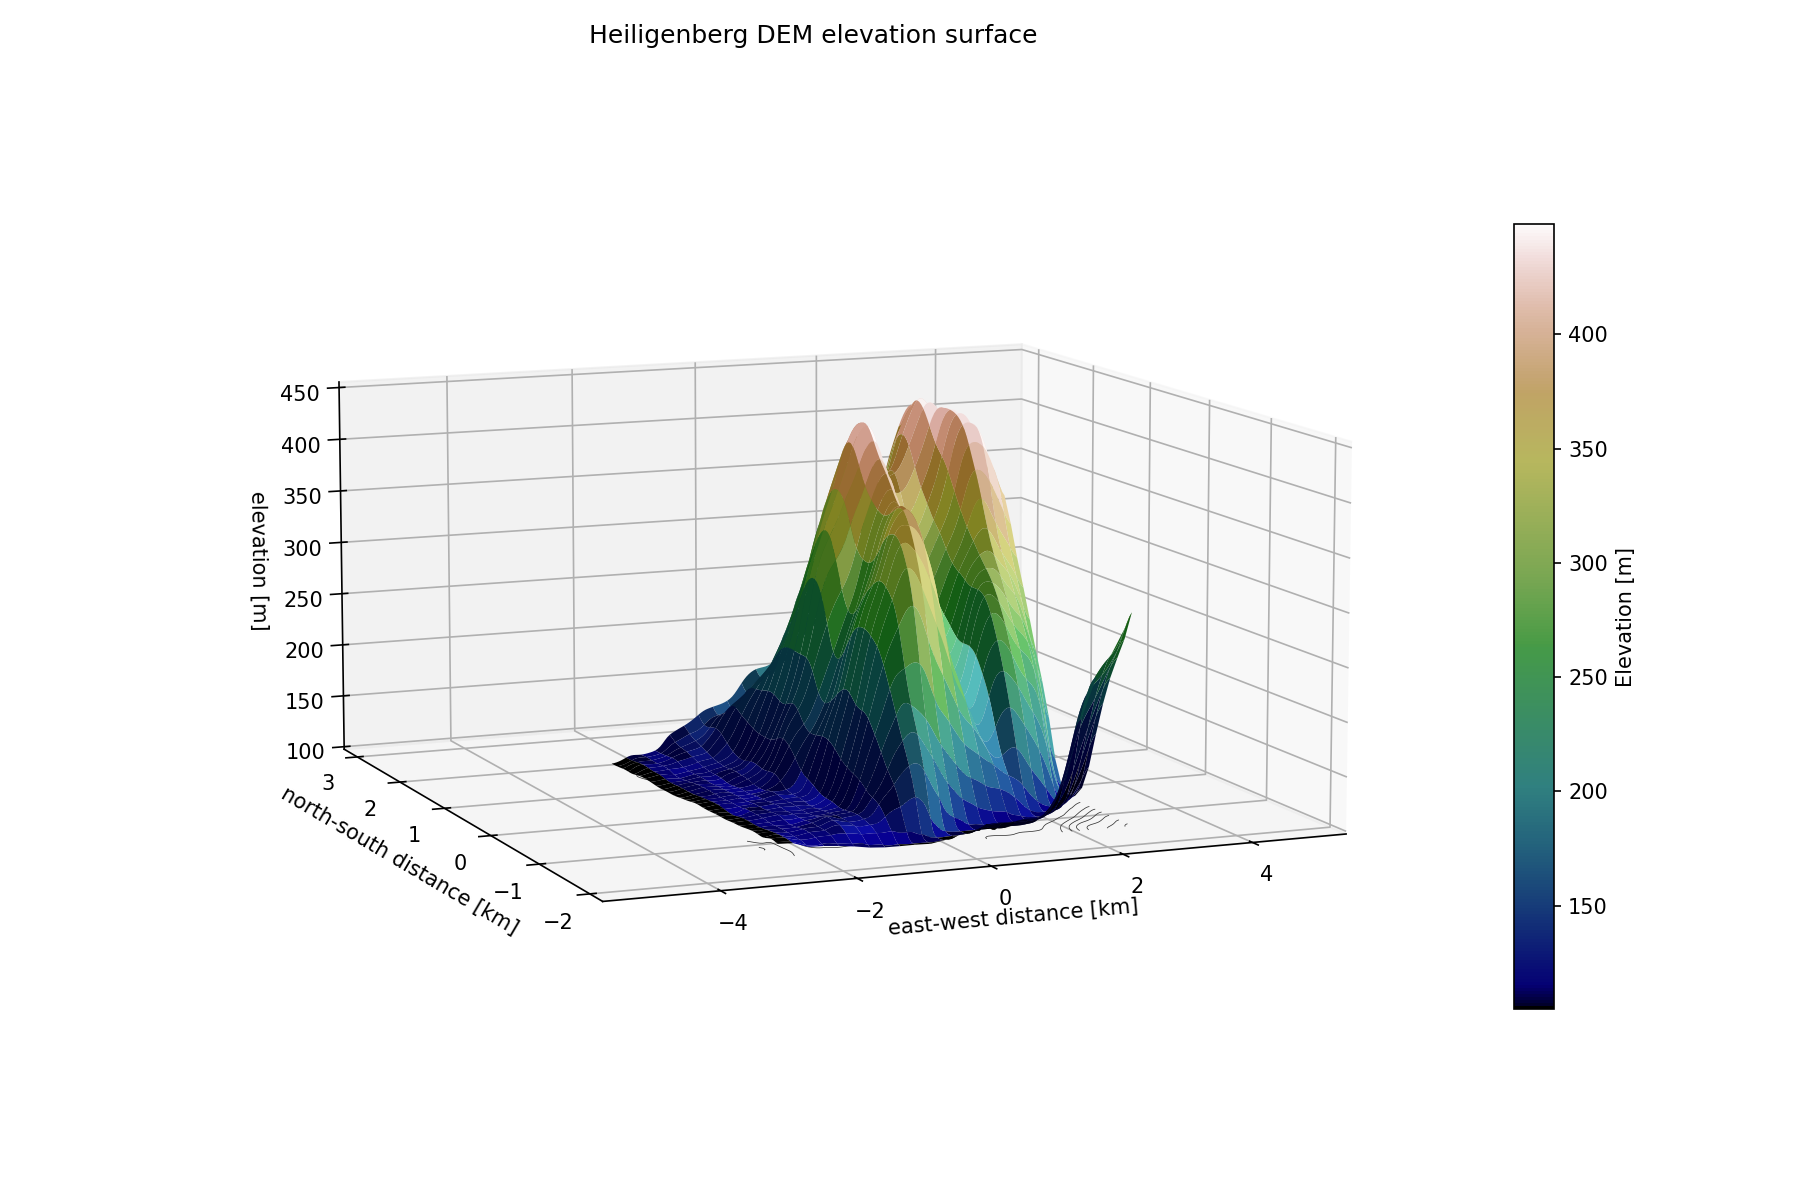
\includegraphics[width=.9\textwidth]{pic/topography_surface}
  \end{center}
\end{frame}

% \begin{frame}{Isoflächen}
%     \begin{columns}
%         \begin{column}{.5\textwidth}
%             \begin{gather*}
%                 f:\R^3\to \R
%             \end{gather*}
%         \end{column}
%         \begin{column}{.5\textwidth}
%             \begin{center}
% %                \includegraphics[width=\textwidth]{fig/Benzene_density_isosurface.png}
%                 Benzol, Elektronendichte
%             \end{center}
%             \tiny Xavier Andrade, CC BY-SA 3.0, via Wikimedia Commons
%         \end{column}
%     \end{columns}
% \end{frame}

\subsection{Partielle Ableitungen}
\mrnote{Provisorisch sind die Folien aus Carl Herrmanns Teil zu partiellen Ableitungen eingefügt}

%%%%%%%%%%%%%%%%%%%%%%%%%%%%%%%%%%%%%%%%%%%%%%%%%%%%%
\begin{frame}
    \frametitle{Partielle Ableitungen}

\begin{itemize}
    \item Eine Raumdimension
    \begin{itemize}
        \item Die Ableitung $\frac{df(t)}{dt}$ beschreibt die {\bf Änderung} von $f(t)$ bei infinitesimalen Veränderungen von $t$
    \end{itemize}
    \item {\bf Partielle Ableitung}: Änderung der Funktion $f(x_1,\ldots,x_n)$ bei infinitesimalen Veränderungen {\bf einer} Variablen, wobei die anderen {\bf konstant} bleiben!
\end{itemize}
    \begin{gather*}
        \frac{f(x_1,\ldots,x_k+h, \ldots, x_n) - f(x_1,\ldots, x_n)}{h} \xrightarrow{h \to 0} \frac{\partial f(x_1,\ldots,x_n)}{\partial x_k}  
    \end{gather*}
\end{frame}
 
%%%%%%%%%%%%%%%%%%%%%%%%%%%%%%%%%%%%%%%%%%%%%%%%%%%%%
\begin{frame}
    \frametitle{Notation}

    \begin{itemize}

        \item Schreibweisen:
        $$
        \frac{\partial f}{\partial x_k}=\partial_{x_k} f =f_{x_k}=f_{k}
        $$
        \item Beispiele:
        \begin{xalignat*}3
            f(x,y) &= x^2+y^2 & \partial_x f &= 2x &\partial_y f &= 2y \\
            f(x,y) &= 3x^2y^3 & \partial_x f &= 6xy^3 & \partial_y f &= 9x^2y^2
        \end{xalignat*}
    \end{itemize}
\end{frame}


%%%%%%%%%%%%%%%%%%%%%%%%%%%%%%%%%%%%%%%%%%%%%%%%%%%%
\begin{frame}
    \frametitle{Mehrfache Ableitungen}

    \begin{itemize}
        \item Wie bei Funktionen einer Variablen können wir mehrfache Ableitungen berechnen
        \item Alle Kombinationen von Variablen sind möglich!
        \item z.B.\ bei $f(x_1,\ldots,x_k)$:
        $$
        f_{ij} = \frac{\partial^2 f}{\partial x_i \partial x_j} =  \frac{\partial}{\partial x_i}\left(\frac{\partial f}{\partial x_j}\right)
        $$
    \end{itemize}
\end{frame}

%%%%%%%%%%%%%%%%%%%%%%%%%%%%%%%%%%%%%%%%%%%%%%%%%%%%%
\begin{frame}
    \frametitle<presentation>{Vertauschung von Ableitungen}

    Bei Mehrfachableitungen spielt die Reihenfolge der Ableitungen (bei den Funktionen, die wir betrachten) keine Rolle! (Satz von Schwarz)
\vspace{1em}

    {\bf Beispiel:} $f(x,y,z) = e^{xy^2}\,\sin z$
    \begin{itemize}
        \item $f_x = y^2\,e^{xy^2}\,\sin z$ , $f_y = 2xy\,e^{xy^2}\,\sin z$
        \item bei doppelten Ableitungen gilt: $f_{xy}=f_{yx}$
    \end{itemize}
    \vspace{3cm}

\end{frame}



%%%%%%%%%%%%%%%%%%%%%%%%%%%%%%%%%%%%%%%%%%%%%%%%%%%%%
\begin{frame}
    \frametitle{Partielle Ableitungen und Tangente}

\begin{center}
    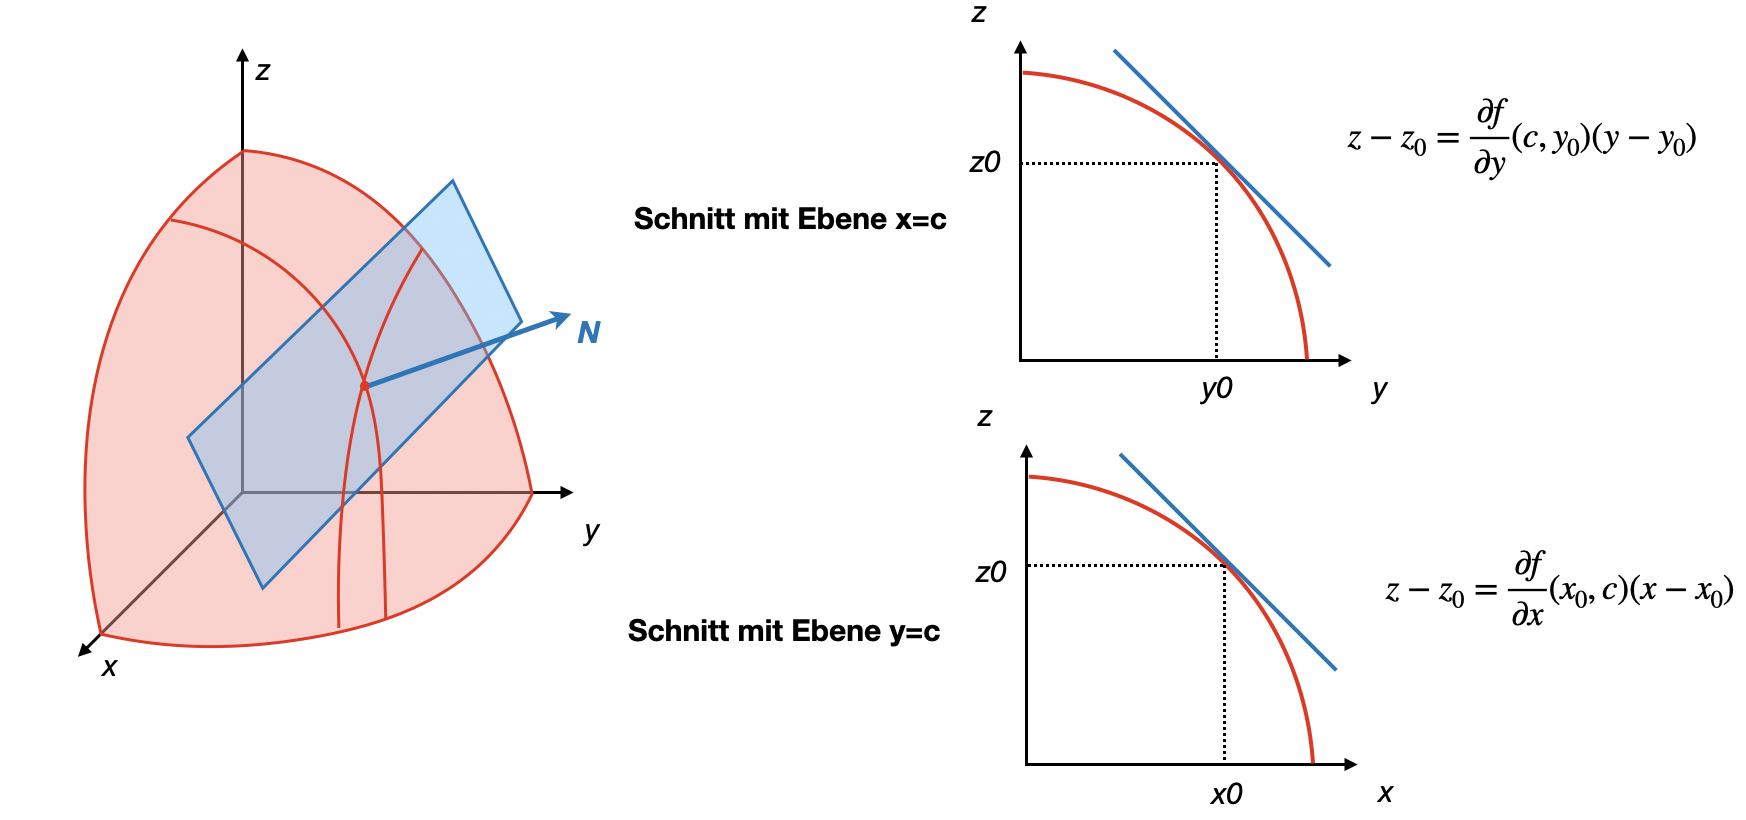
\includegraphics[width=.8\textwidth]{fig/mv10.png}
\end{center}
\begin{itemize}
    \item Gleichung der Tangentialebene am Punkte $(x_0,y_0)$:
    \begin{gather*}
    z-z_0 = \frac{\partial f}{\partial x}(x_0,y_0) (x-x_0) +\frac{\partial f}{\partial y}(x_0,y_0) (y-y_0)         
    \end{gather*}
    \item Normalenvektor zur Ebene:
    $$
    N = (\frac{\partial f}{\partial x}(x_0,y_0), \frac{\partial f}{\partial y}(x_0,y_0),-1)
    $$
\end{itemize}
\end{frame}

%%%%%%%%%%%%%%%%%%%%%%%%%%%%%%%%%%%%%%%%%%%%%%%%%%%%%
\begin{frame}
    \frametitle{Beispiel}

    Wir berechnen die Gleichung der Tangentialebene für die Funktion $z=x^2-y-xe^y$ am Punkt $(x_0,y_0) = (1,0)$:
    \begin{eqnarray*}
    f_x = 2x-e^y &;& f_x(1,0) = 1 \\
    f_y = -1-xe^y &;& f_y(1,0) = -2
    \end{eqnarray*}
    Da $z_0=f(1,0) = 0$ gilt folgende Gleichung:
    $$
    z -z_0 = f_x(1,0)(x-1) + f_y(1,0)(y-0) \iff z = x-1 -2y 
    $$

    Normalenvektor:
    $$
    N = (1,-2,-1)
    $$
\end{frame}

%%%%%%%%%%%%%%%%%%%%%%%%%%%%%%%%%%%%%%%%%%%%%%%%%%%%%
\begin{frame}
    \frametitle{Gradient einer Funktion}

    \begin{itemize}
        \item Wir definieren den {\bf Gradienten} der Funktion $f$:
        $$
    \nabla f = \left(\begin{array}{c} \partial_{x_1}f \\ \vdots \\  \partial_{x_n}f \end{array}\right)
        $$
        \item $\nabla f(p)$ ist ein Vektor in $\mathbb{R}^n$ am Punkt $p$
        \item Beispiel: $f(x,y) = 3x^2y^3$:
        $$
        \nabla f = \left(\begin{array}{c} 6xy^3 \\ 9x^2y^2 \end{array}\right) ~~\rightarrow~~ \nabla f(1,1) = \left(\begin{array}{c} 6 \\ 9 \end{array}\right)
        $$
\end{itemize}
\end{frame}

%%%%%%%%%%%%%%%%%%%%%%%%%%%%%%%%%%%%%%%%%%%%%%%%%%%%%%%%%%%%
%%%%%%%%%%%%%%%%%%%%%%%%%%%%%%%%%%%%%%%%%%%%%%%%%%%%%%%%%%%%
\subsection{Richtungsableitungen}

\begin{frame}
    \frametitle{Veränderungen in beliebige Richtungen}

    \begin{itemize}
        \item Die partiellen Ableitungen $\partial_x f$ unf $\partial_y f$ beschreiben die Veränderungen von $z=f(x,y)$ wenn man sich in $x-$ bzw $y-$Richtung bewegt
        \item Wie verändert sich die Funktion, wenn man sich in eine beliebige Richtung bewegt?
        \item Richtung gegeben durch Vektor $\vu$
        \item {\bf Richtungsableitung} (in 2 Dimensionen):
        $$
        D_u f = \frac{\partial f}{\partial x}\cdot u_1 + \frac{\partial f}{\partial y}\cdot u_2
        $$
    \end{itemize}
    \begin{center}
        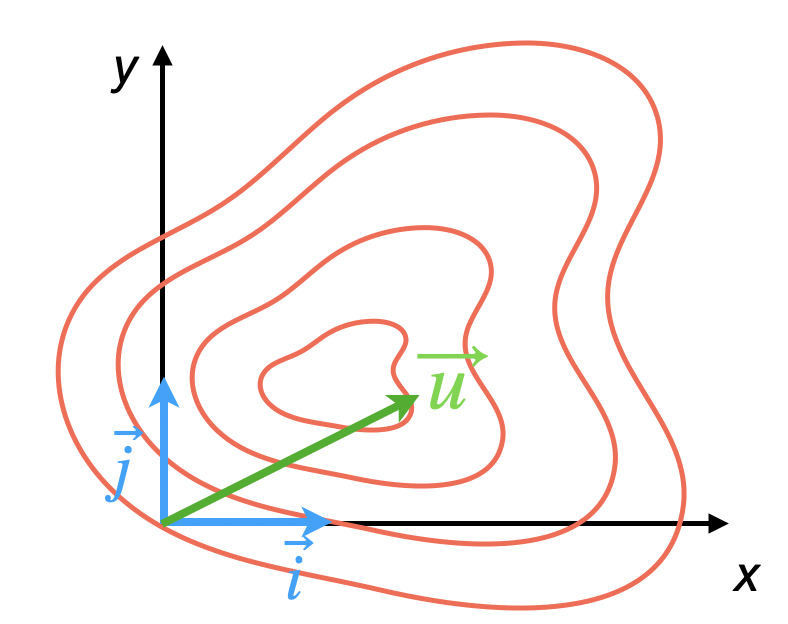
\includegraphics[width=.3\textwidth]{img/mv17.png}
    \end{center}

\end{frame}

%%%%%%%%%%%%%%%%%%%%%%%%%%%%%%%%%%%%%%%%%%%%%%%%%%%%%
\begin{frame}
    \frametitle{Richtungsableitung}

    \begin{itemize}
        \item Schreibweise mit Gradient (Skalarprodukt!):
        $$
        D_u f = \nabla f \cdot \vu
        $$
        \item $D_u f(p)$ gibt an, wie stark die Steigung in $\vu$-Richtung am Punkt $p$ ist
        \item $D_u f(p)>0$ bzw. $D_u f(p)< 0$: es geht nach oben bzw.\ nach unten!
          \pause
        \item Die Richtungsableitung hängt von der Länge des Richtungsvektors ab
          \begin{itemize}
          \item Manche Autoren fordern $\left|\vu\right| = 1$
          \item Wir normieren bei Bedarf
          \end{itemize}
    \end{itemize}
\end{frame}

%%%%%%%%%%%%%%%%%%%%%%%%%%%%%%%%%%%%%%%%%%%%%%%%%%%%%
\begin{frame}
    \frametitle{Richtung konstanter Werte}

    \begin{center}
        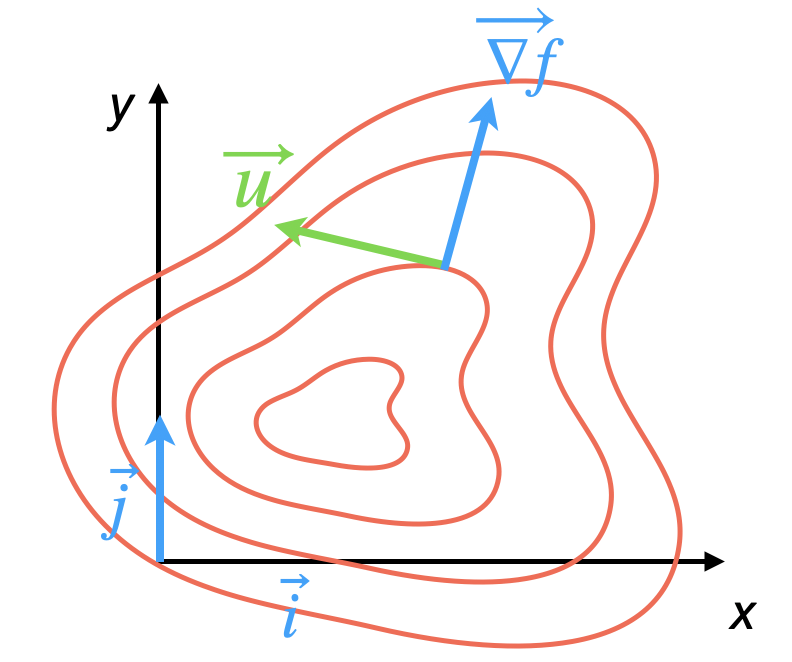
\includegraphics[width=.3\textwidth]{img/mv18.png}
    \end{center}

    \begin{itemize}
        \item In welche Richtung verändert sich die Funktion {\bf nicht}?
        $$
        D_u f = 0 ~\iff~ \nabla f \cdot \vu =0 ~\iff ~ \nabla f \perp \vu
        $$
        \item $\vu$ ist ein {\bf Tangentialvektor} zu den Höhenlinien!
    \end{itemize}
\end{frame}
%%%%%%%%%%%%%%%%%%%%%%%%%%%%%%%%%%%%%%%%%%%%%%%%%%%%%
\begin{frame}
    \frametitle{Abstiegs- und Aufstiegsrichtungen}

    \begin{center}
        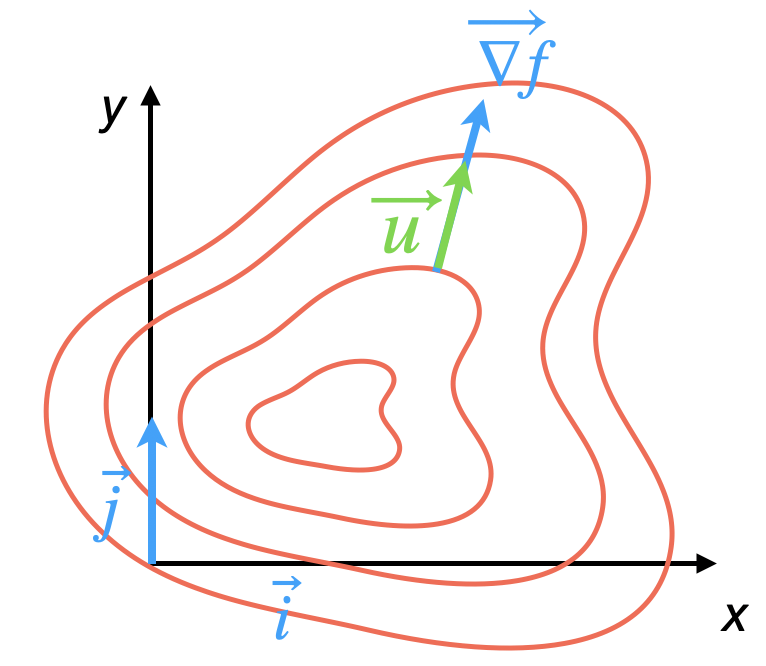
\includegraphics[width=.3\textwidth]{img/mv19.png}
    \end{center}

    \begin{itemize}
        \item In welche Richtung ist die Veränderung {\bf am größten}?
        $$
        \max_{\vu} D_u f ~\iff ~ \vu \parallel\nabla f
        $$
        \item Wenn $\vu$ Einheitsvektor: $\vu=\frac{\nabla f}{|\nabla f|}$; daher
        $
        D_u f = \nabla f \cdot \frac{\nabla f}{|\nabla f|} = |\nabla f|
        $
        \item Der Gradient gibt an jedem Punkt die Richtung der {\bf größten Veränderung} (orthogonal zu den  Höhenlinien)
    \end{itemize}
\end{frame}

%%%%%%%%%%%%%%%%%%%%%%%%%%%%%%%%%%%%%%%%%%%%%%%%%%%%%
\begin{frame}
    \frametitle{Beispiel}

    \begin{itemize}
        \item $f(x,y) = \frac{1}{2}(14-x^2-y^2)$
        \item Gradient:
          \begin{gather*}
            \nabla f =
            \begin{pmatrix}
              -x\\-y
            \end{pmatrix}
          \end{gather*}
        \item Am Punkt $(x_0,y_0) = (1,2)$: $z_0 = \nicefrac92$
        $$
        \nabla f (x_0,y_0) = \left(\begin{array}{c}-1 \\ -2\end{array}\right)
        $$

        \end{itemize}
    \end{frame}

   %%%%%%%%%%%%%%%%%%%%%%%%%%%%%%%%%%%%%%%%%%%%%%%%%%%%%
   \begin{frame}
    \frametitle<presentation>{Beispiel}

    \begin{itemize}
        \item Größte Steigung am Punkt $(x_0,y_0)$:
        $$
            |\nabla f (x_0,y_0)| = \sqrt{\left(-1\right)^2+\left(-2\right)^2} = \sqrt{5}
        $$
        \item Richtung der Höhenlinien: entlang der Höhenlinien ist die Steigung Null; daher erfüllt der Tangentialvektor zu den Höhenlinien die Bedingung:
        $$
        \nabla f (x_0,y_0)\cdot \vu = 0 ~\iff~ \vu ~~\parallel~~ \left(\begin{array}{c}2 \\ -1\end{array}\right)
        $$
        \item Einheitsvektor:  $\vec{e}_u = \frac{\vu}{|\vu|} ~\Rightarrow~ \vec{e}_u= \frac{1}{\sqrt{5}}\left(\begin{array}{c}2 \\ -1\end{array}\right) $
    \end{itemize}
\end{frame}

        \item Die Fläche eines Dreiecks ist gegeben durch $A(a,b,\theta) = \frac{1}{2}ab\sin\theta$; bestimmen Sie das totale Differential  !
        \item Das Volumen eines Zylinders ist $V=\pi r^2 h$; verändert sich das Volumen mehr, wenn $r$ von $1.0$ auf $1.1$ oder $h$ von $1.0$ auf $1.1$ erhöht wird?
    \end{enumerate}
\end{frame}

%%%%%%%%%%%%%%%%%%%%%%%%%%%%%%%%%%%%%%%%%%%%%%%%%%%%%%%%%%%%
\begin{frame}{Ableitung entlang eines Weges}
  \begin{itemize}
  \item Wir bewegen uns entlang eines Weges $\vx(t)$ im Raum
  \item Im Raum ist eine differenzierbare Funktion $f(\vx)$ definiert
  \item Wie ändert sich der Wert dieser Funktion abhängig von $t$?
  \item Kettenregel:
    \begin{gather*}
      \frac{d}{dt} f(\vx(t)) = \nabla f(\vx(t)) \cdot \vx'(t)
    \end{gather*}
  \end{itemize}
\end{frame}

%%%%%%%%%%%%%%%%%%%%%%%%%%%%%%%%%%%%%%%%%%%%%%%%%%%%%%%%%%%%
\begin{frame}{Beispiel}
  \begin{gather*}
    f(\vx) = \tfrac12(x^2+y^2),\qquad
    \nabla f =
    \begin{pmatrix}
      x\\y
    \end{pmatrix}
  \end{gather*}
  \begin{itemize}
  \item Kreislinie:
    \begin{gather*}
      \vx(t) =
      \begin{pmatrix}
        \cos t\\\sin t
      \end{pmatrix},
      \qquad
      \vx'(t) =
      \begin{pmatrix}
        -\sin t\\\cos t
      \end{pmatrix},
      \qquad
      \nabla f(\vx)\cdot \vx'(t) = 0
    \end{gather*}
    \pause
  \item Gerade durch null:
    \begin{gather*}
      \vx = \sqrt2
      \begin{pmatrix}
        t\\t
      \end{pmatrix},\qquad
      \vx'(t) =
      \begin{pmatrix}
        1\\1
      \end{pmatrix},
      \qquad
      \nabla f(\vx)\cdot \vx'(t) = t
    \end{gather*}
  \end{itemize}
\end{frame}

\begin{envgknote}{Neue Struktur}
    \begin{itemize}
    \item Höhenlinien- und Schnittliniendiagramme (Vorlesung 3.1)
    \item Isoflächen, Orbitale?
    \item Partielle Ableitungen, Gradient, Richtungsableitungen
    \item Extremwertaufgaben über Variationsprinzip (Vorlesung 3.4)
    \item Gradient Descent (Vorlesung 3.6)
    \item Optimierung mittels Lagrange-Multiplikatoren (Vorlesung 3.7)
    \end{itemize}
\end{envgknote}

\begin{envmrerror}{Ergänzungen aus der aktuellen Vorlesung}
\begin{itemize}
    \item Schnittliniendiagramme (Vorlesung 3.1)
    \item Fehlerfortpflanzung additiver und multiplikativer Fehler (Vorlesung 3.3). Hier könnte überlegt werden, ob ausgehend von der bestehenden Vorlesung ein Übergang zum Kapitel 4 \textit{Auswirkung von Eingabe- und Rechenfehlern} gemacht werden könnte.
    \item Extremwertaufgaben, Hesse-Matrix, Definitheit von Matrizen (Vorlesung 3.4)
    \item Optimierung mittels Lagrange-Multiplikatoren (Vorlesung 3.7)
    \item Richtungsableitungen (Vorlesung 3.5)    
    \item Gradient Descent (Vorlesung 3.6)
\end{itemize}
\end{envmrerror}

\begin{envmrnote}{Mögliche Klausuraufgaben}
\begin{itemize}
    \item Zuordnung von Höhenlinien/Schnittlinien-Diagrammen zu Plots von Funktionen
    \item Analyse und Interpretation von Funktionen anhand von gegebenen Höhenlinien/Schnittliniendiagrammen oder selbstständig geeignete Höhen/Schnittebenen zur Funktionsanalyse finden und diese Auswahl begründen
\end{itemize}
\end{envmrnote}

  

\mode<all>
